\section{Design of the System}
\label{sec:SystemDesign}


%later convert this pdf
\begin{figure}[t]
\centering
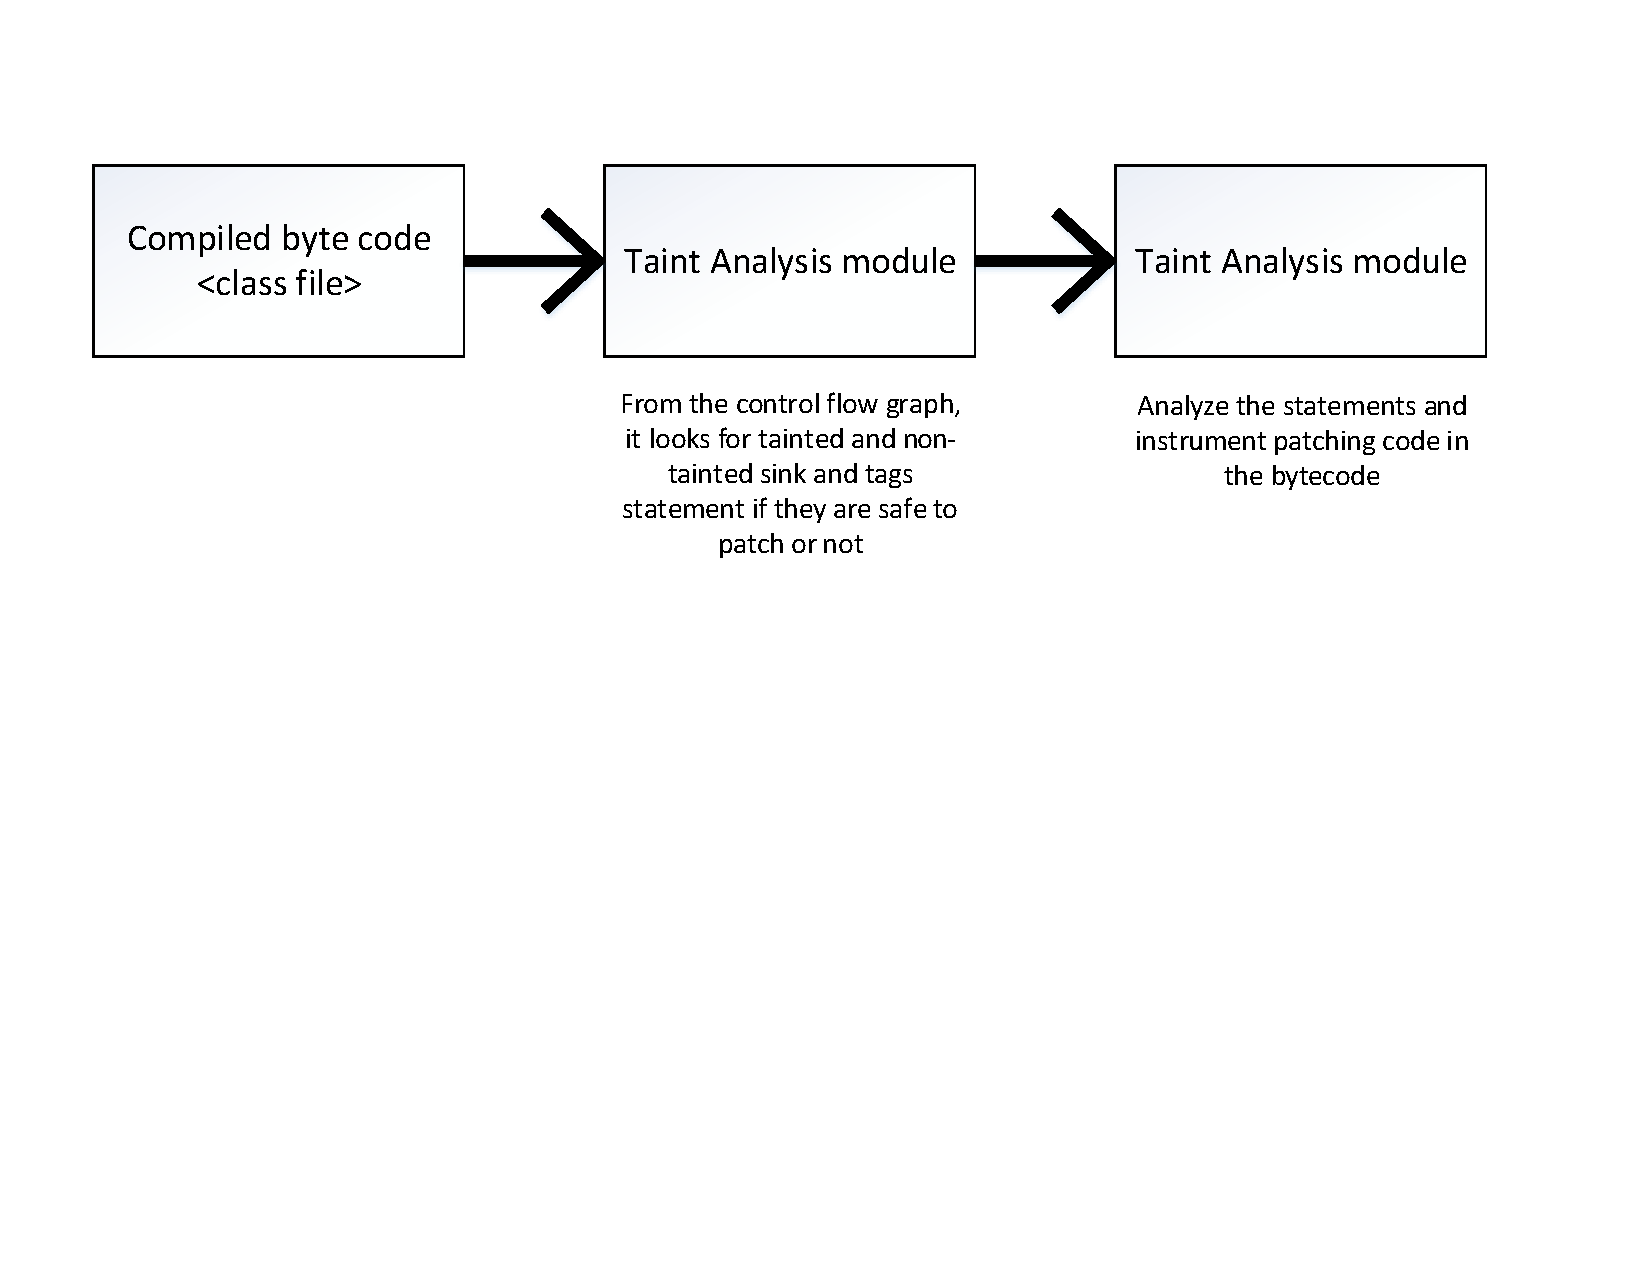
\includegraphics[scale=.42]{images/OverallDesign.pdf}
\caption{Overall Design}
\label{fig:overallDesign}
\end{figure}


% \begin{figure}[!htb]
% \centering
% 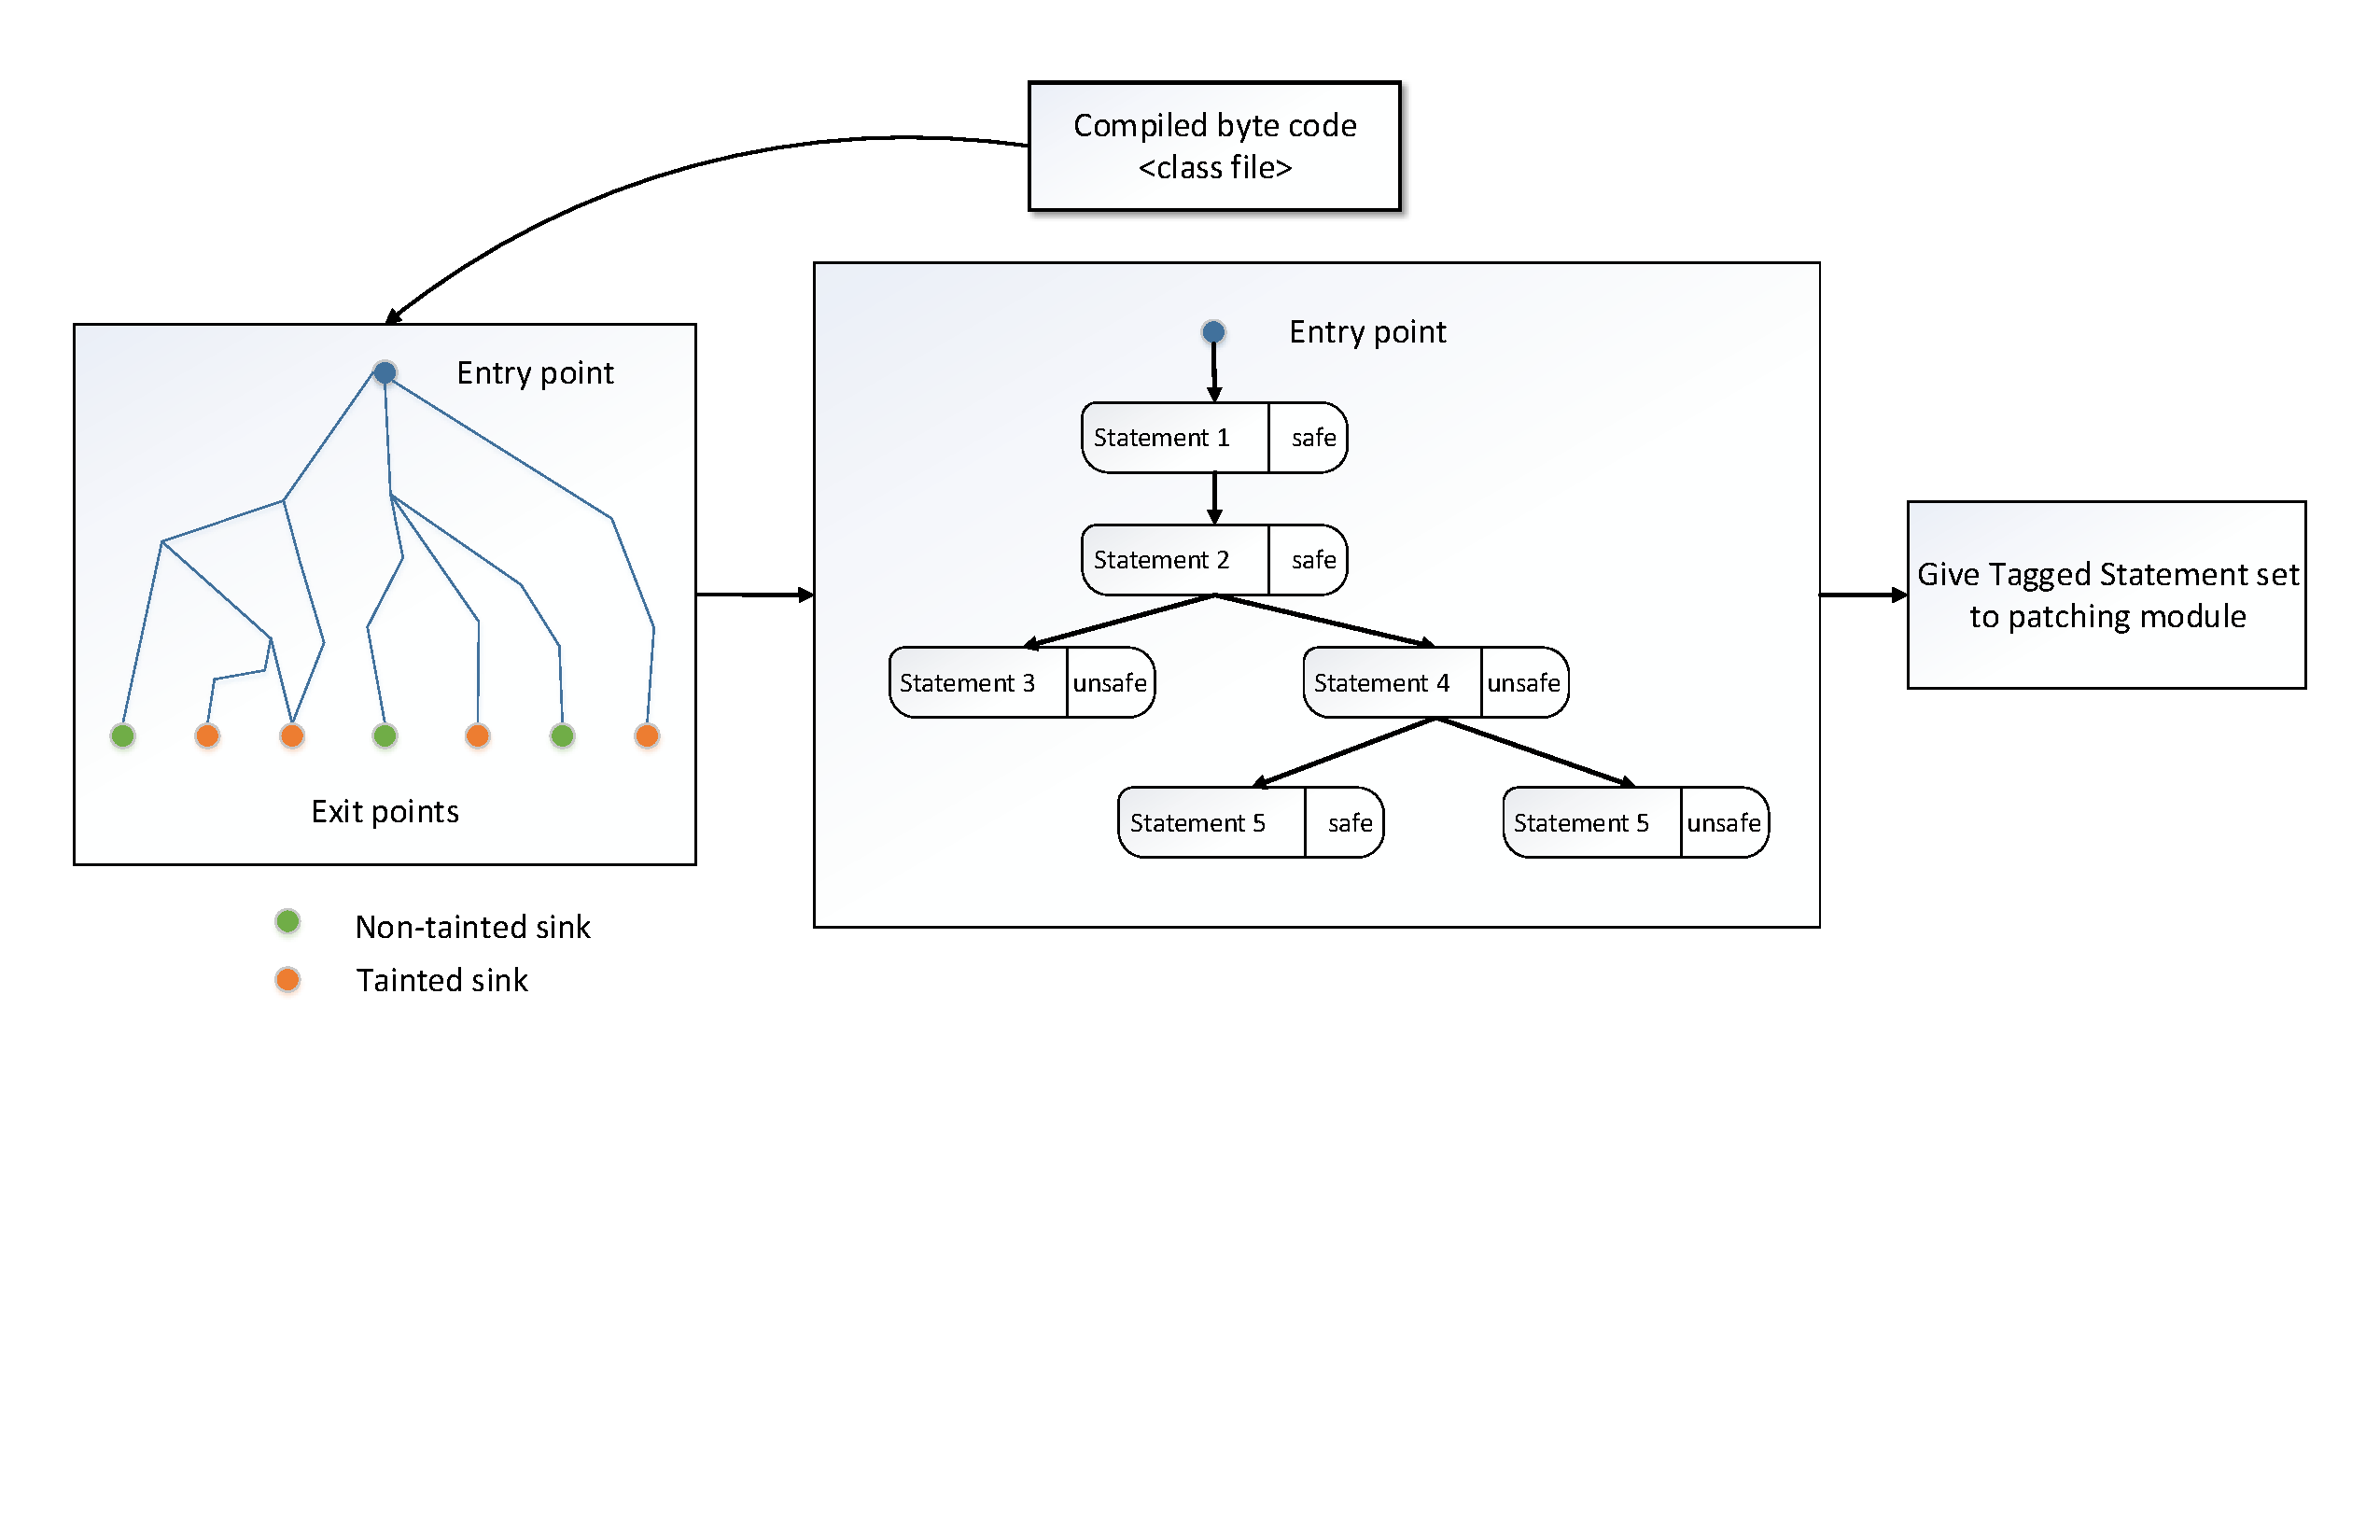
\includegraphics[width=3.5in]{images/TaintModule.pdf}
% \caption{Overall Design}
% \label{fig:TaintModule}
% \end{figure}
% 
% \begin{figure*
%   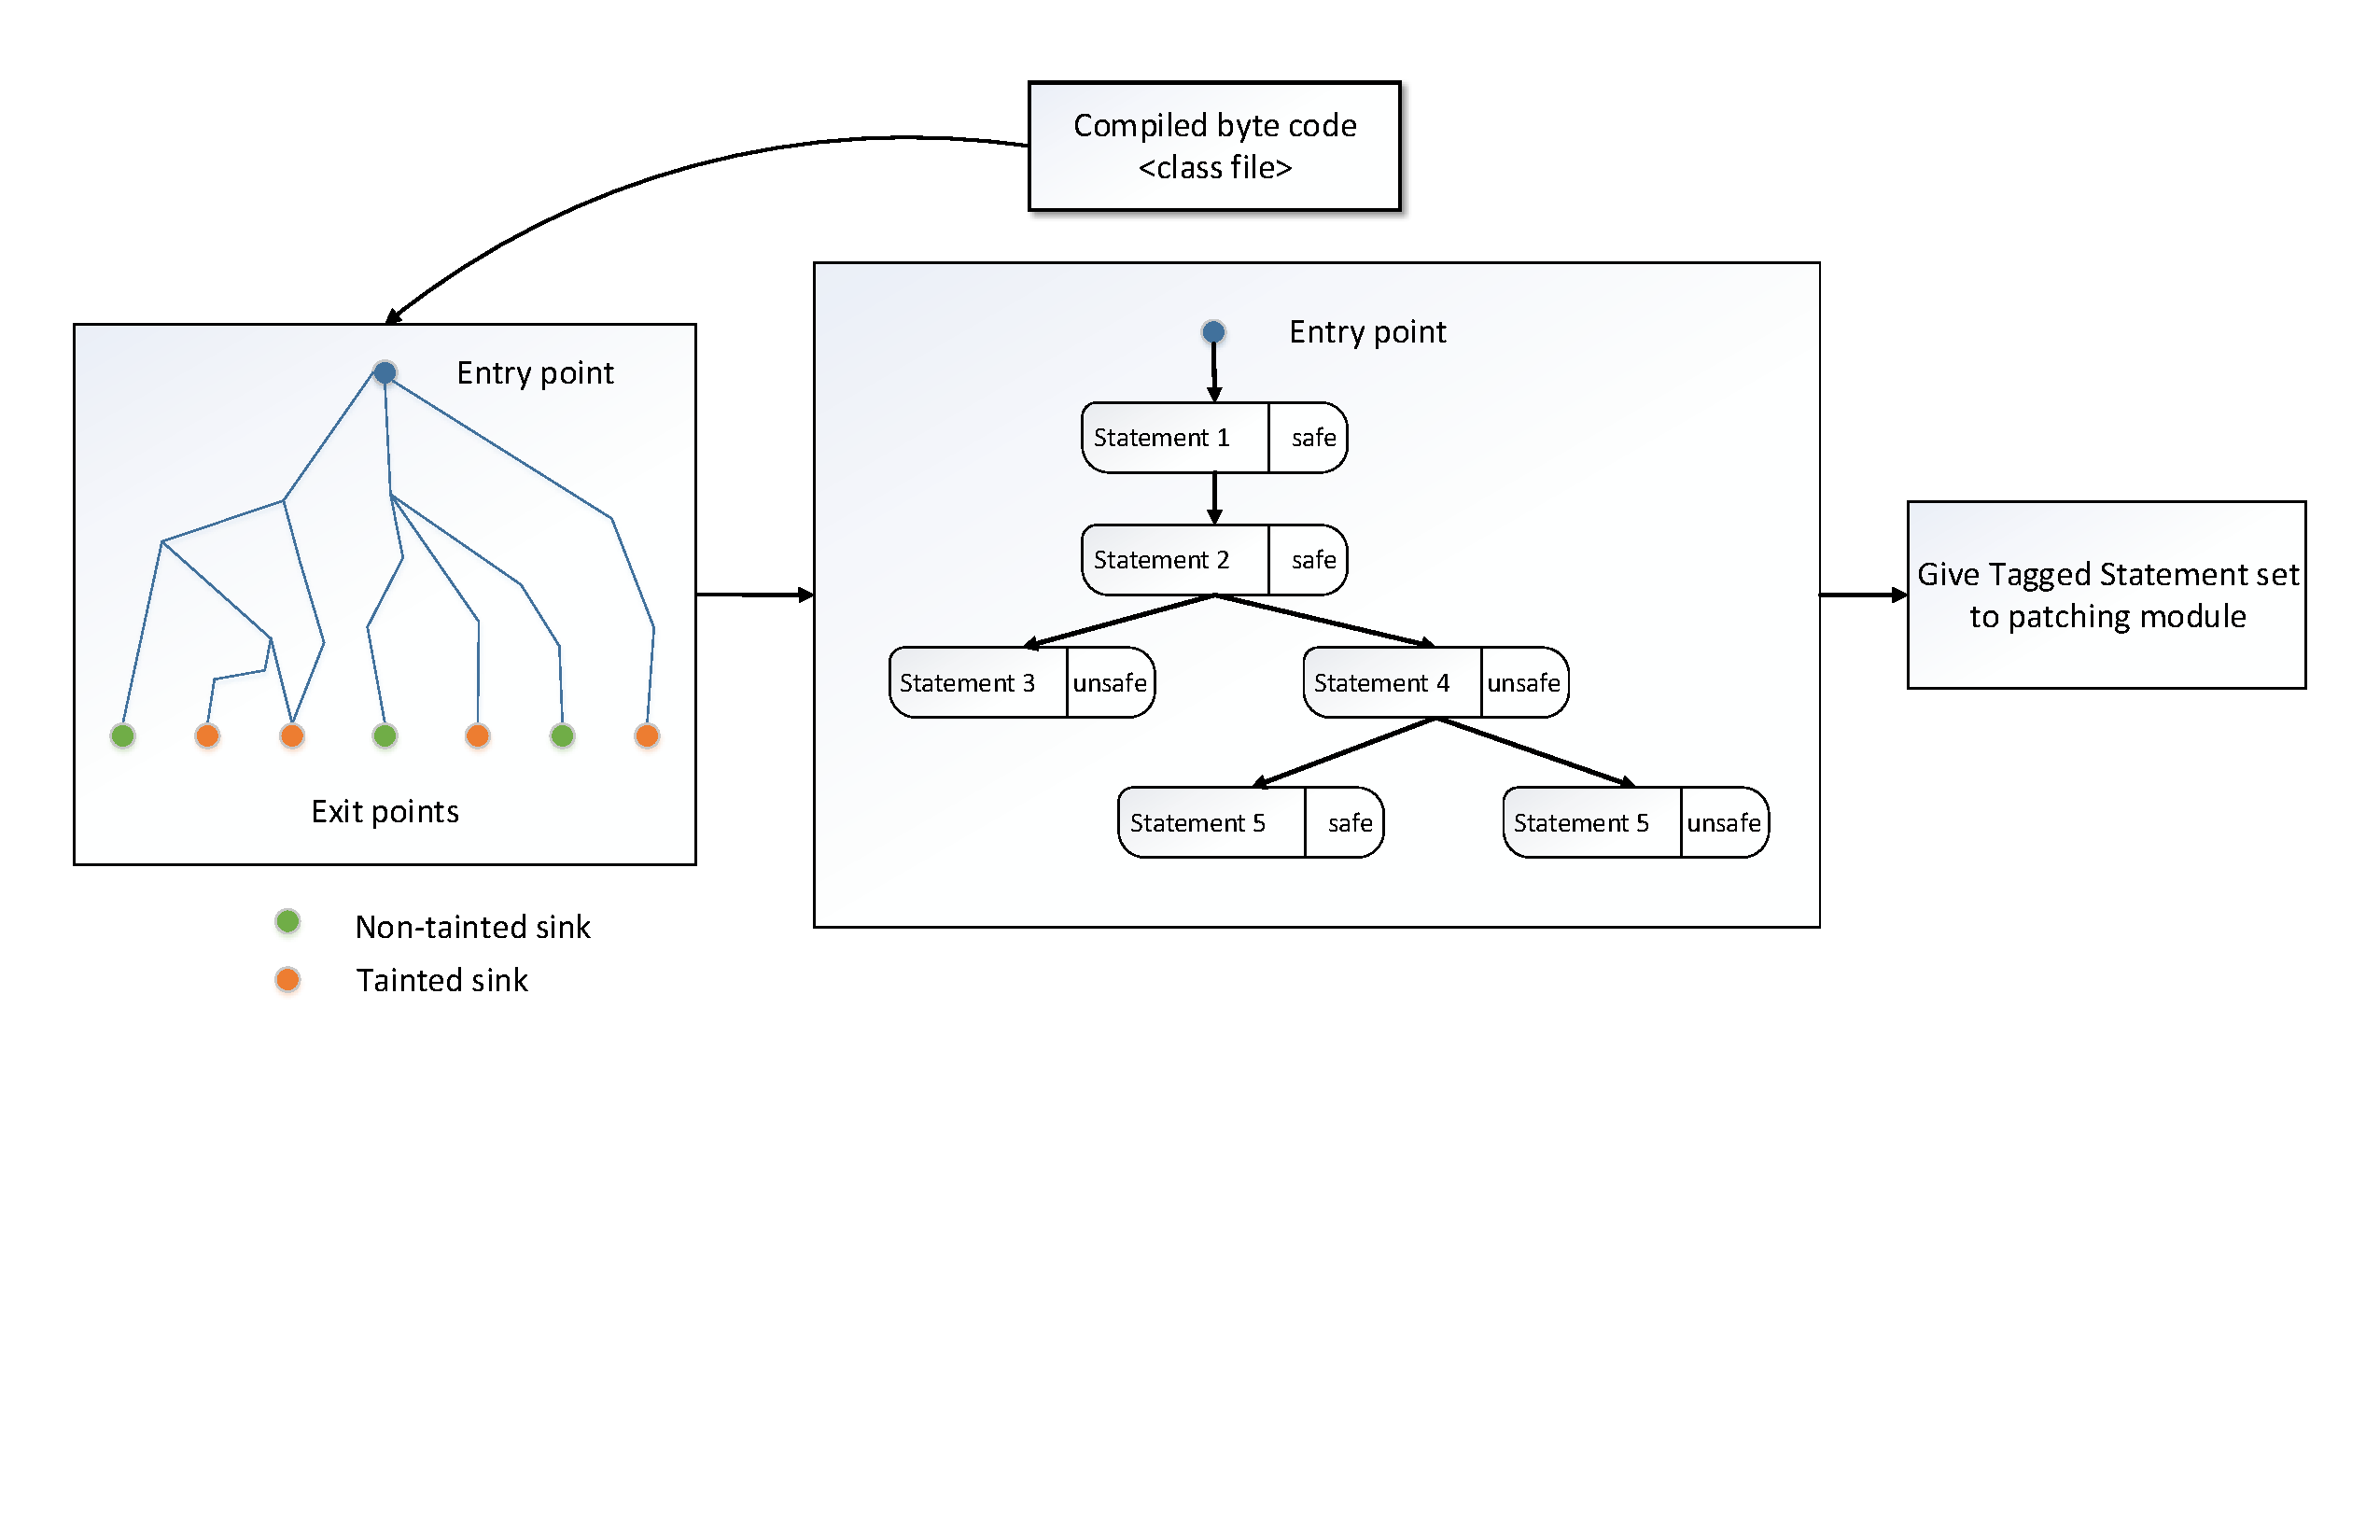
\includegraphics[width=\textwidth,height=5cm]{images/TaintModule.pdf}
%   \caption{Design of the Taint Module}
% \end{figure*}

%later covert this to pdf
\begin{figure*}[t]
\centering
  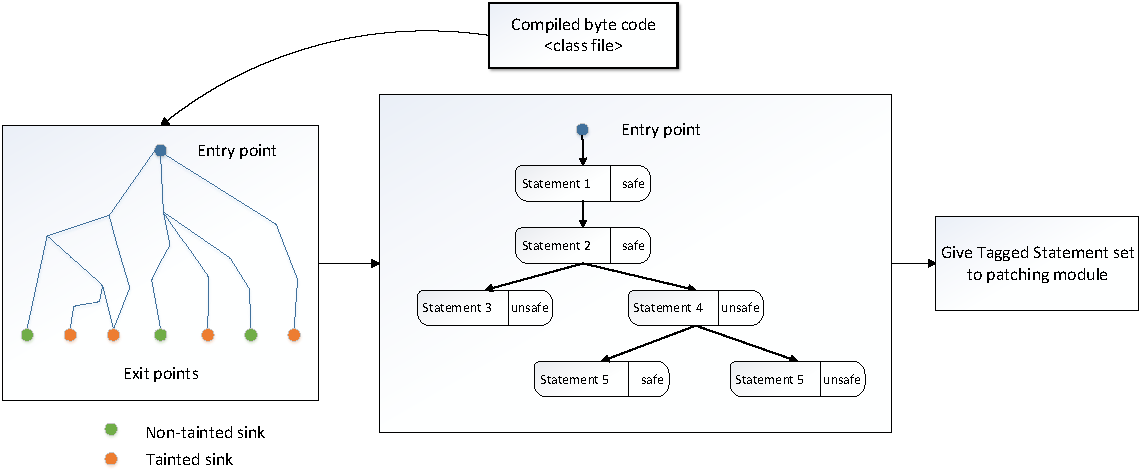
\includegraphics[scale= .4]{images/TaintModule.png}
  \caption{Design of the Taint Module}
  \label{fig:TaintModule}
\end{figure*}


The overall design of the repairing framework is illustrated in
Figure~\ref{fig:overallDesign}. The framework consists of four basic modules.


\subsection{Taint analysis Module}
\label{subsec:TaintModule}

The main purpose of the taint analysis module is to classify which of the
statements are safe to patch or not. Based on the analysis result in this
module, the tagged statement will be passed to the repairing module.


We have specify the list of source, sink and derivation methods in a
configuration file before the analysis. The source methods includes methods
which
take input from user from console or web application forms like text box. The
sink methods are sensitive data storage which are unsafe to manipulate such as
database, console print or methods to send a text file to printer etc. The
overview of the taint analysis module is illustrated in the
Figure~\ref{fig:TaintModule}.  The input for the module is the compiled byte
code intended to be repaired. Here we have generated a control flow graph (CFG)
from to get all the possible program paths. The module will return all the
program statements which are on any of the program paths from source to sink.


\subsubsection{Tainting Rules}
\label{subsubsec:TaintingRule}
%\textcolor{red}{\textbf{Needs Revision}}\newline

\begin{table}[t]
\centering
\small
\begin{tabular}{l|l}
\multicolumn{1}{c|}{\textbf{\java\ Class}} & \multicolumn{1}{c}{\textbf{Source
Method}}\\
% \scalebox{0.86}
% {
\hline
\code{java.io.InputStream} & \code{read()}\\
\code{java.io.BufferedReader} & \code{readLine()}\\
\code{java.net.URL} & \code{openConnection()}\\
\code{org.apache.http.HttpResponse} & \code{getEntity()}\\
\code{org.apache.http.util.EntityUtils} & \code{toString()}\\
\code{org.apache.http.util.EntityUtils} & \code{toByteArray()}\\
\code{org.apache.http.util.EntityUtils} & \code{getContentCharSet()}\\
\code{javax.servlet.http.HttpServletRequest} & \code{getParameter()}\\
\code{javax.servlet.ServletRequest} & \code{getParameter()}\\
\code{java.Util.Scanner} & \code{next()}\\
\end{tabular}
\caption{Common \java\ library taint source functions}
\label{tab:TaintSources}
% }
\end{table}



\begin{table}[t]
\centering
\small
\begin{tabular}{l|l}
\multicolumn{1}{c|}{\textbf{\java\ Class}} & \multicolumn{1}{c}{\textbf{Sink
Method}}\\
% \scalebox{0.86}
% {
\hline
\code{java.io.PrintStream} & \code{printf()}\\
\code{java.io.OutputStream} & \code{write()}\\
\code{java.io.FileOutputStream} & \code{write()}\\
\code{java.io.Writer} & \code{write()}\\
\code{java.net.Socket} & \code{connect()}\\
%org.apache.http.impl.client.DefaultHttpClient & execute\\ \hline
\end{tabular}
% }
\caption{Common \java\ library taint sink functions}
\label{tab:TaintSinks}
\end{table}

~\newline

For any generic taint analysis, the tainting rules including a list of source 
and sink is to be defined. For our analysis we applied these policies, 

\begin{mylist}
  \item We defined list of source and sink taint methods listed in
  Table~\ref{tab:TaintSources} and \ref{tab:TaintSinks}. We are only tainting
  the variables which are coming from the listed taint source methods.
  
  \item We have also listed all taint propagation methods. The assignment ($=$)
  is the basic taint propagator. But there are other methods like \code{append}
  in \code{java.lang.StringBuffer} and \code{java.lang.StringBuilder} which are
  taint propagator.

  \item All the variable which are referred to tainted variables/ objects or
  output of taint propagator over tainted variable/objects are also considered
  as tainted.

  \item For all the program patch we see if such tainted variables are reaching
  the tainted sink or not. If they are reaching to some tainted sink then all
  the statements along that particular program path to which the tainted
  variables are assigned are marked as unsafe otherwise safe.
\end{mylist}


\subsection{Repairing Module}
\label{subsec:RepairingModule}

%later covert this to pdf
\begin{figure}[t]
\centering
  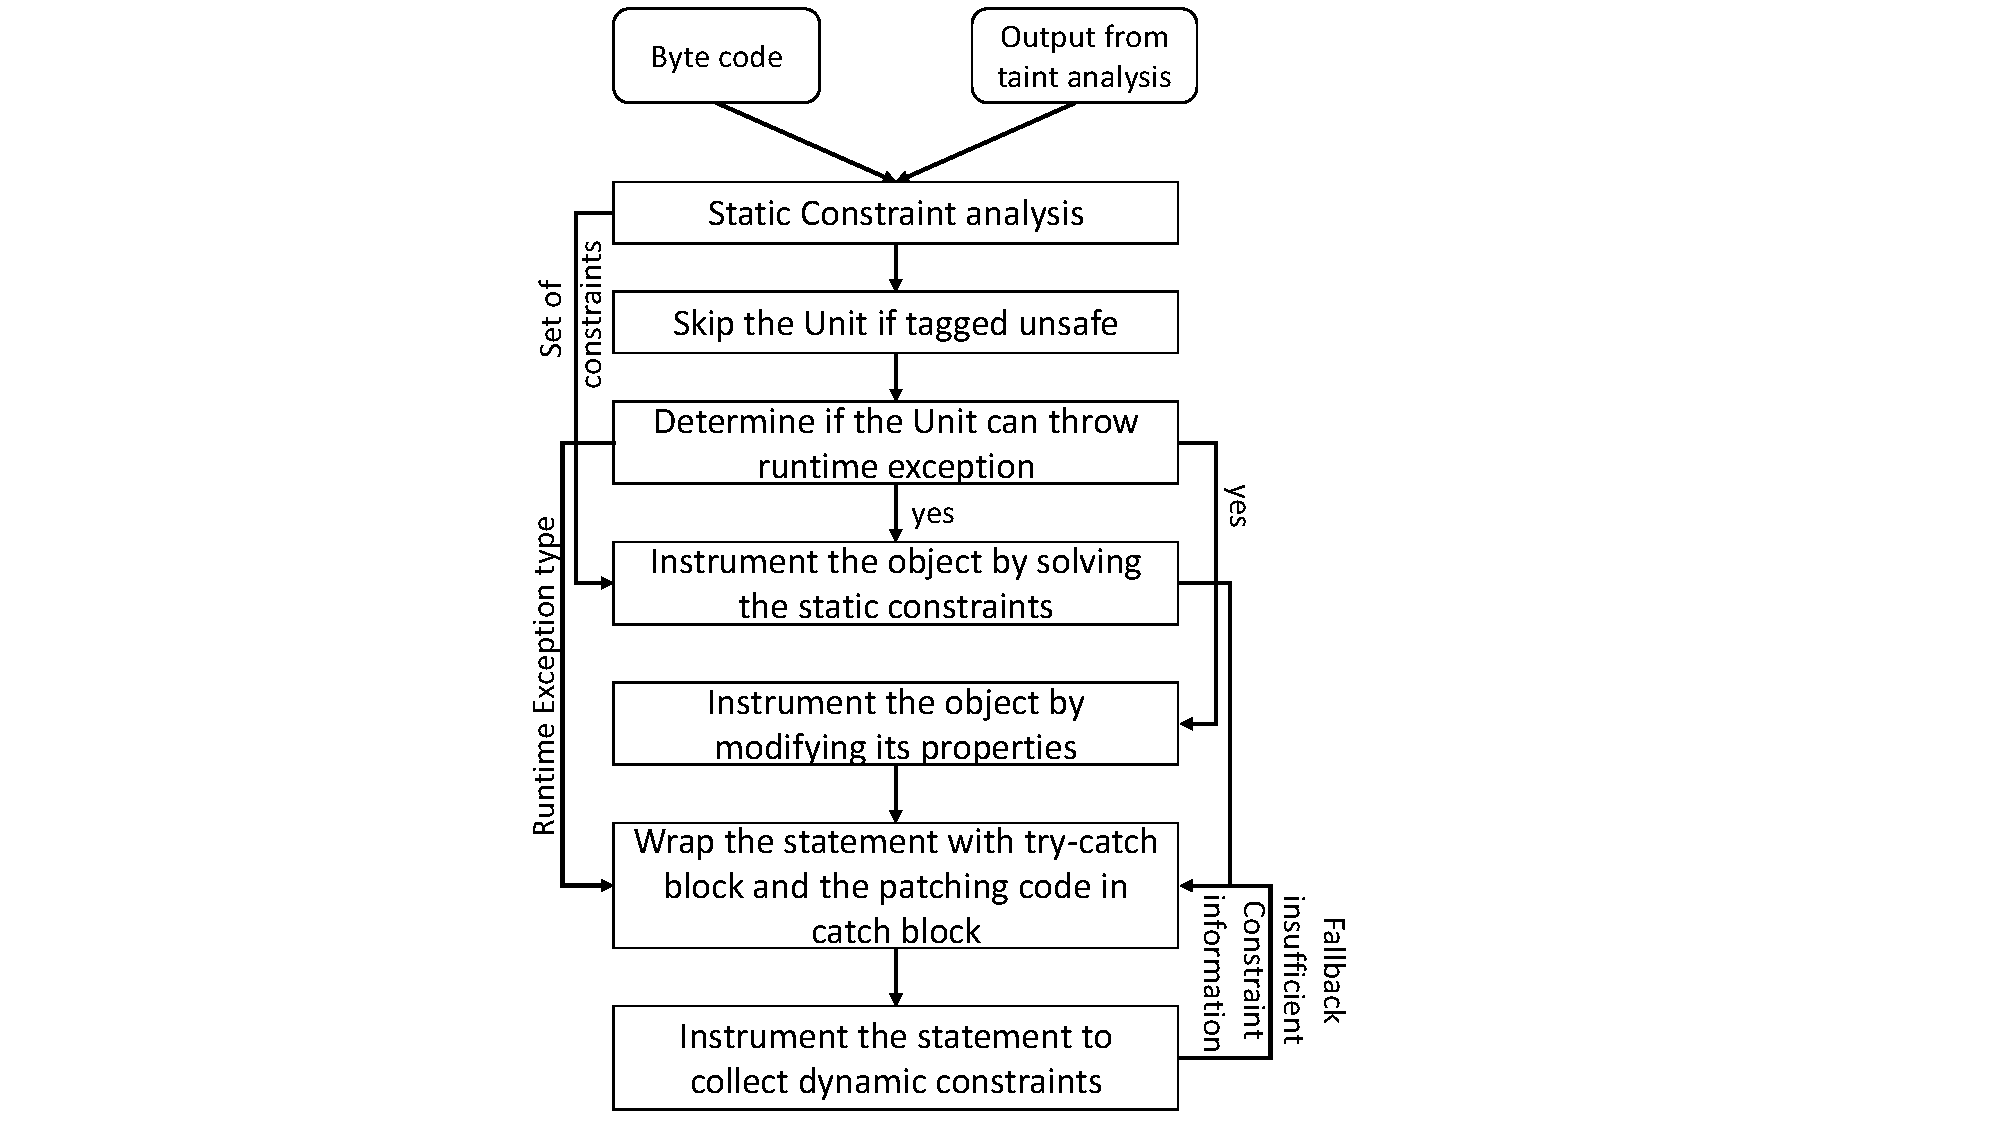
\includegraphics[scale= .4]{images/PatchModule.pdf}
  \caption{Design of the Patching Module}
  \label{fig:PatchModule}
\end{figure}

The repairing module is consisted of three phases. All these three phases
requires three sequential passes over the input bytecodes to produce the final
patched result.